\documentclass[usenames,dvipsnames]{beamer}
\usepackage{../../shared/styles/custom}
\usepackage{../../shared/styles/conventions}
\usepackage{tikz}
\usepackage{pdfpages}
\usetikzlibrary{arrows.meta, positioning, decorations.pathreplacing}

% Define expectation command
\newcommand{\E}{\mathbb{E}}

\title{Gradient Descent: The Foundation of Machine Learning}
\subtitle{From Taylor Series to Modern Deep Learning}
\date{\today}
\author{Nipun Batra and the teaching staff}
\institute{IIT Gandhinagar}

\begin{document}
  \maketitle

  \begin{frame}{Table of Contents}
    \tableofcontents
  \end{frame}

  \section{Introduction: Why Optimization Matters}
  
  \begin{frame}{The Core Machine Learning Challenge}
    \begin{keypointsbox}
    \textbf{Central Problem:} Find the best parameters $\vtheta^*$ for our model
    \end{keypointsbox}
    
    \pause
    \textbf{Examples everywhere in ML:}
    \begin{itemize}[<+->]
        \item \textbf{Linear regression:} $\min_{\vtheta} \|\vy - \mX\vtheta\|^2$
        \item \textbf{Logistic regression:} $\min_{\vtheta} -\sum \log p(y_i|\vx_i, \vtheta)$
        \item \textbf{Neural networks:} $\min_{\vtheta} \sum \ell(f(\vx_i; \vtheta), y_i)$
    \end{itemize}
    
    \pause
    \begin{alertbox}{The Challenge}
    Most ML problems have \textbf{no closed-form solution!}
    \end{alertbox}
  \end{frame}

  \begin{frame}{Enter: Iterative Optimization}
    \textbf{Since we can't solve directly, we use iterative methods:}
    
    \begin{center}
    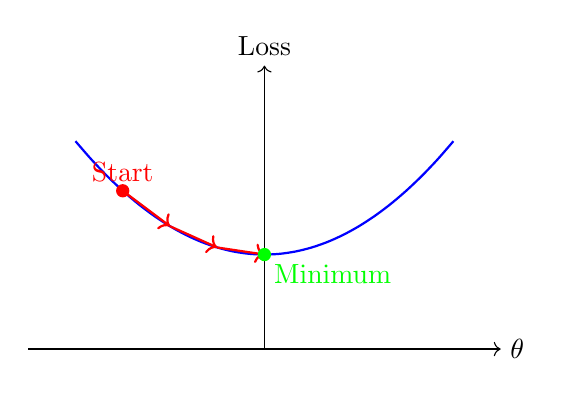
\begin{tikzpicture}[scale=1.2]
      % Draw a simple loss landscape
      \draw[thick, domain=-2:2, smooth, variable=\x, blue] plot ({\x}, {0.3*\x*\x + 1});
      \draw[->] (-2.5,0) -- (2.5,0) node[right] {$\theta$};
      \draw[->] (0,0) -- (0,3) node[above] {Loss};
      
      % Show iterative steps
      \fill[red] (-1.5, {0.3*(-1.5)*(-1.5) + 1}) circle (2pt) node[above] {Start};
      \draw[->, thick, red] (-1.5, {0.3*(-1.5)*(-1.5) + 1}) -- (-1, {0.3*(-1)*(-1) + 1});
      \draw[->, thick, red] (-1, {0.3*(-1)*(-1) + 1}) -- (-0.5, {0.3*(-0.5)*(-0.5) + 1});
      \draw[->, thick, red] (-0.5, {0.3*(-0.5)*(-0.5) + 1}) -- (0, 1);
      \fill[green] (0, 1) circle (2pt) node[below right] {Minimum};
    \end{tikzpicture}
    \end{center}
    
    \pause
    \begin{definitionbox}{Gradient Descent}
    The workhorse algorithm that powers modern machine learning
    \end{definitionbox}
  \end{frame}

  \section{Intuition: Following the Steepest Path}

  \begin{frame}{The Mountain Climbing Analogy}
    \textbf{Imagine: You're lost in fog and want to reach the valley}
    
    \begin{center}
    \begin{tikzpicture}[scale=1.5]
      % Draw mountain-like curve
      \draw[thick, domain=-3:3, smooth, variable=\x, blue] 
        plot ({\x}, {0.1*(\x+2)*(\x+2)*(\x-1)*(\x-1) + 0.5});
      
      % Add person and arrows showing steepest descent
      \fill[red] (-1, {0.1*(-1+2)*(-1+2)*(-1-1)*(-1-1) + 0.5}) circle (2pt);
      \draw[->, thick, red, line width=2pt] 
        (-1, {0.1*(-1+2)*(-1+2)*(-1-1)*(-1-1) + 0.5}) -- 
        (-0.5, {0.1*(-0.5+2)*(-0.5+2)*(-0.5-1)*(-0.5-1) + 0.5})
        node[midway, above] {\small Steepest descent};
        
      \node[red] at (-1, {0.1*(-1+2)*(-1+2)*(-1-1)*(-1-1) + 0.5 + 0.3}) {\small You};
      \node at (1, 2) {\textcolor{blue}{Loss landscape}};
    \end{tikzpicture}
    \end{center}
    
    \pause
    \textbf{Strategy:} Always step in the steepest \textcolor{red}{downhill} direction
  \end{frame}

  \begin{frame}{Mathematical Definition of Gradient}
    \begin{center}
    \includegraphics[scale=0.7]{../../maths/assets/mathematical-ml/figures/contour-x_squared_plus_y_squared_quiver-with-gradient.pdf}
    \end{center}
    
    \textbf{For function $f(x, y) = x^2 + y^2$:}
    
    \pause
    \begin{definitionbox}{Gradient}
    $$\nabla f(x, y) = \begin{bmatrix} \frac{\partial f}{\partial x} \\ \frac{\partial f}{\partial y} \end{bmatrix} = \begin{bmatrix} 2x \\ 2y \end{bmatrix}$$
    \end{definitionbox}
    
    \pause
    \begin{keypointsbox}
    \textbf{Key insight:} Gradient points in direction of steepest \textcolor{red}{ascent}
    
    So $-\nabla f$ points in direction of steepest \textcolor{blue}{descent}!
    \end{keypointsbox}
  \end{frame}

  \section{Mathematical Foundation: Taylor Series}

  \begin{frame}{Why Taylor Series?}
    \begin{examplebox}{The Core Idea}
    If we can't solve $\min f(\vx)$ exactly, let's approximate $f(\vx)$ locally!
    \end{examplebox}
    
    \pause
    \textbf{Taylor series expansion around point $\vx_0$:}
    
    \begin{align}
        f(\vx) &= f(\vx_0) + \nabla f(\vx_0)^T(\vx-\vx_0) + \frac{1}{2}(\vx-\vx_0)^T\nabla^2 f(\vx_0)(\vx-\vx_0) + \ldots
    \end{align}
    
    \pause
    \textbf{Different orders of approximation:}
    \begin{itemize}[<+->]
        \item \textbf{0th order:} $f(\vx) \approx f(\vx_0)$ (constant)
        \item \textbf{1st order:} $f(\vx) \approx f(\vx_0) + \nabla f(\vx_0)^T(\vx-\vx_0)$ (linear)
        \item \textbf{2nd order:} Includes curvature via Hessian
    \end{itemize}
  \end{frame}

  \begin{frame}{Taylor Series: Concrete Example}
    \textbf{Let's approximate} $f(x) = \cos(x)$ \textbf{around} $x_0 = 0$:
    
    \begin{itemize}[<+->]
        \item $f(0) = \cos(0) = 1$
        \item $f'(0) = -\sin(0) = 0$  
        \item $f''(0) = -\cos(0) = -1$
        \item $f'''(0) = \sin(0) = 0$
        \item $f^{(4)}(0) = \cos(0) = 1$
    \end{itemize}
    
    \pause
    \textbf{Taylor approximations:}
    \begin{align}
        \text{0th:} \quad &f(x) \approx 1\\
        \text{2nd:} \quad &f(x) \approx 1 - \frac{x^2}{2}\\
        \text{4th:} \quad &f(x) \approx 1 - \frac{x^2}{2} + \frac{x^4}{24}
    \end{align}
  \end{frame}

  \begin{frame}{Visual: Taylor Approximations}
    \begin{center}
    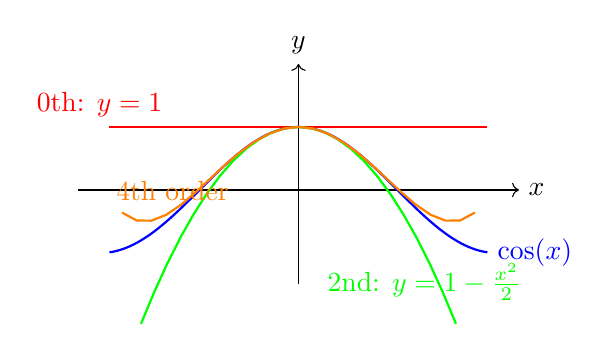
\begin{tikzpicture}[scale=0.8]
      \draw[->] (-3.5,0) -- (3.5,0) node[right] {$x$};
      \draw[->] (0,-1.5) -- (0,2) node[above] {$y$};
      
      % Original function cos(x)
      \draw[thick, blue, domain=-3:3, samples=100] plot (\x, {cos(\x r)}) 
        node[right] {$\cos(x)$};
      
      % 0th order approximation
      \draw[thick, red, domain=-3:3] plot (\x, 1) 
        node[above left] at (-2,1) {0th: $y=1$};
      
      % 2nd order approximation  
      \draw[thick, green, domain=-2.5:2.5] plot (\x, {1 - \x*\x/2}) 
        node[below] at (2, {1-2}) {2nd: $y=1-\frac{x^2}{2}$};
      
      % 4th order approximation
      \draw[thick, orange, domain=-2.8:2.8] plot (\x, {1 - \x*\x/2 + \x*\x*\x*\x/24}) 
        node[above] at (-2, {1 - 4/2 + 16/24}) {4th order};
    \end{tikzpicture}
    \end{center}
    
    \begin{keypointsbox}
    Higher-order = better approximation, but 1st-order is often sufficient!
    \end{keypointsbox}
  \end{frame}

  \section{Derivation: From Taylor Series to Gradient Descent}

  \begin{frame}{The Key Question}
    \textbf{Goal:} Find $\Delta \vx$ such that $f(\vx_0 + \Delta \vx) < f(\vx_0)$
    
    \pause
    \textbf{Using 1st-order Taylor approximation:}
    \begin{align}
        f(\vx_0 + \Delta \vx) &\approx f(\vx_0) + \nabla f(\vx_0)^T \Delta \vx
    \end{align}
    
    \pause
    \textbf{For the function to decrease:}
    $$\nabla f(\vx_0)^T \Delta \vx < 0$$
    
    \pause
    \begin{alertbox}{Vector Geometry Reminder}
    For vectors $\mathbf{a}, \mathbf{b}$: $\mathbf{a}^T\mathbf{b} = |\mathbf{a}||\mathbf{b}|\cos(\theta)$
    
    \textbf{Most negative when:} $\cos(\theta) = -1$ (opposite directions!)
    \end{alertbox}
  \end{frame}

  \begin{frame}{Visual Derivation with TikZ}
    \begin{center}
    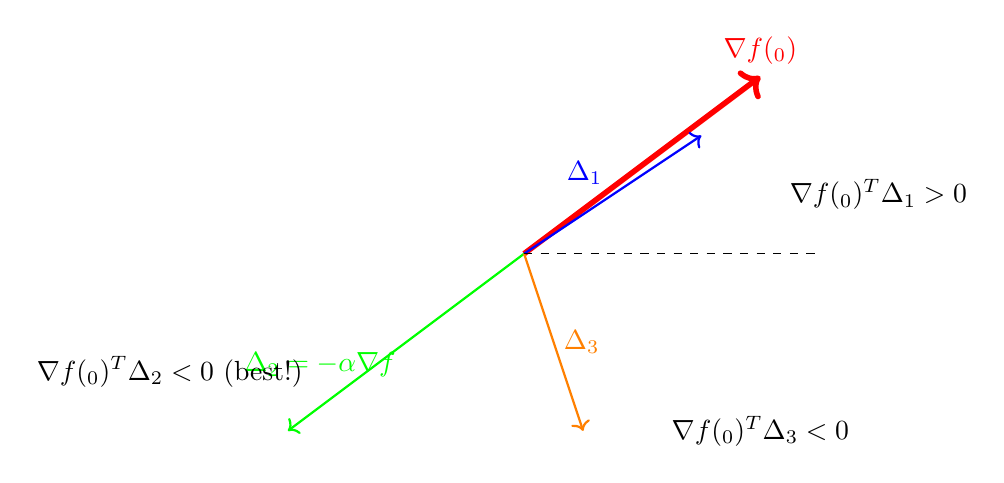
\begin{tikzpicture}[scale=1.5]
      % Draw gradient vector
      \draw[->, thick, red, line width=2pt] (0,0) -- (2,1.5) 
        node[above] {$\nabla f(\vx_0)$};
      
      % Draw potential step directions
      \draw[->, thick, blue] (0,0) -- (1.5,1) 
        node[midway, above left] {$\Delta \vx_1$};
      \draw[->, thick, green] (0,0) -- (-2,-1.5) 
        node[midway, below left] {$\Delta \vx_2 = -\alpha \nabla f$};
      \draw[->, thick, orange] (0,0) -- (0.5,-1.5) 
        node[midway, right] {$\Delta \vx_3$};
      
      % Show angles
      \draw[dashed] (0,0) -- (2.5,0);
      \node at (3, 0.5) {$\nabla f(\vx_0)^T \Delta \vx_1 > 0$};
      \node at (-3, -1) {$\nabla f(\vx_0)^T \Delta \vx_2 < 0$ (best!)};
      \node at (2, -1.5) {$\nabla f(\vx_0)^T \Delta \vx_3 < 0$};
    \end{tikzpicture}
    \end{center}
    
    \pause
    \begin{definitionbox}{Optimal Choice}
    $$\Delta \vx = -\alpha \nabla f(\vx_0), \quad \alpha > 0$$
    \end{definitionbox}
    
    \pause
    \textbf{This gives us the gradient descent update:}
    $$\vx_{\text{new}} = \vx_{\text{old}} - \alpha \nabla f(\vx_{\text{old}})$$
  \end{frame}

  \stepcounter{popquiz}
  \begin{frame}{Pop Quiz \#\thepopquiz: Understanding the Derivation}
    \begin{popquizbox}{\thepopquiz}
    Consider $f(x) = x^2 + 2$ at point $x_0 = 2$.
    
    \textbf{Questions:}
    \begin{enumerate}
        \item What is $f(x_0)$ and $f'(x_0)$?
        \item Write the 1st-order Taylor approximation
        \item If we take step $\Delta x = -0.1 \cdot f'(x_0)$, what is our new $x$?
        \item Will the function value decrease?
    \end{enumerate}
    \end{popquizbox}
  \end{frame}

  \section{The Gradient Descent Algorithm}

  \begin{frame}{The Complete Algorithm}
    \begin{definitionbox}{Gradient Descent Algorithm}
    An iterative first-order optimization method for finding local minima
    \end{definitionbox}
    
    \pause
    \textbf{Algorithm Steps:}
    \begin{enumerate}[<+->]
        \item \textbf{Initialize:} Choose starting point $\vtheta_0$
        \item \textbf{Repeat until convergence:}
        \begin{itemize}
            \item Compute gradient: $\vg_t = \nabla f(\vtheta_t)$
            \item Update parameters: $\vtheta_{t+1} = \vtheta_t - \alpha \vg_t$  
            \item Check stopping criterion
        \end{itemize}
    \end{enumerate}
    
    \pause
    \textbf{Key hyperparameter: Learning rate $\alpha$}
  \end{frame}

  \begin{frame}{Learning Rate: The Step Size}
    \textbf{The learning rate $\alpha$ controls how big steps we take:}
    
    \begin{itemize}[<+->]
        \item \textbf{Too small $\alpha$:} Slow convergence
        \item \textbf{Good $\alpha$:} Fast, stable convergence  
        \item \textbf{Too large $\alpha$:} Overshooting, instability
        \item \textbf{Way too large $\alpha$:} Divergence!
    \end{itemize}
    
    \pause
    \begin{keypointsbox}
    Learning rate selection is crucial for success!
    \end{keypointsbox}
  \end{frame}

  \begin{frame}{Learning Rate Visualization: Too Small}
    \textbf{$\alpha = 0.01$ - Slow but steady}
    \begin{center}
    \includegraphics[scale=0.6]{../../maths/assets/mathematical-ml/figures/gd-lr-0.01.pdf}
    \end{center}
    
    \begin{alertbox}{Issue}
    Many iterations needed → Computationally expensive
    \end{alertbox}
  \end{frame}

  \begin{frame}{Learning Rate Visualization: Just Right}
    \textbf{$\alpha = 0.1$ - The sweet spot}
    \begin{center}
    \includegraphics[scale=0.6]{../../maths/assets/mathematical-ml/figures/gd-lr-0.1.pdf}
    \end{center}
    
    \begin{keypointsbox}
    Perfect balance: Fast convergence + Stability
    \end{keypointsbox}
  \end{frame}

  \begin{frame}{Learning Rate Visualization: Too Large}
    \textbf{$\alpha = 0.8$ - Getting risky}
    \begin{center}
    \includegraphics[scale=0.6]{../../maths/assets/mathematical-ml/figures/gd-lr-0.8.pdf}
    \end{center}
    
    \begin{alertbox}{Warning}
    Fast but oscillatory - watch for instability!
    \end{alertbox}
  \end{frame}

  \begin{frame}{Learning Rate Visualization: Disaster}
    \textbf{$\alpha = 1.01$ - Complete failure}
    \begin{center}
    \includegraphics[scale=0.6]{../../maths/assets/mathematical-ml/figures/gd-lr-1.01.pdf}
    \end{center}
    
    \begin{alertbox}{Disaster Zone}
    Function values explode! Always monitor your loss curves.
    \end{alertbox}
  \end{frame}

  \section{Application: Linear Regression}

  \begin{frame}{Our First Real Example}
    \textbf{Problem:} Learn $y = \theta_0 + \theta_1 x$ from data
    
    \begin{center}
    \begin{tabular}{|c|c|}
        \hline
        \textbf{x} & \textbf{y} \\
        \hline
        1 & 1 \\
        2 & 2 \\
        3 & 3 \\
        \hline
    \end{tabular}
    \end{center}
    
    \pause
    \textbf{Cost function (Mean Squared Error):}
    $$\MSE(\theta_0, \theta_1) = \frac{1}{n}\sum_{i=1}^n (y_i - \hat{y}_i)^2$$
    $$= \frac{1}{n}\sum_{i=1}^n (y_i - \theta_0 - \theta_1 x_i)^2$$
  \end{frame}

  \begin{frame}{Computing the Gradients}
    \textbf{We need:} $\nabla \MSE = \begin{bmatrix} \frac{\partial \MSE}{\partial \theta_0} \\ \frac{\partial \MSE}{\partial \theta_1} \end{bmatrix}$
    
    \pause
    \textbf{Partial derivatives:}
    
    \begin{align}
        \frac{\partial \MSE}{\partial \theta_0} &= \frac{2}{n}\sum_{i=1}^n (y_i - \theta_0 - \theta_1 x_i)(-1)\\
        &= -\frac{2}{n}\sum_{i=1}^n \epsilon_i
    \end{align}
    
    \pause
    \begin{align}
        \frac{\partial \MSE}{\partial \theta_1} &= \frac{2}{n}\sum_{i=1}^n (y_i - \theta_0 - \theta_1 x_i)(-x_i)\\
        &= -\frac{2}{n}\sum_{i=1}^n \epsilon_i x_i
    \end{align}
    
    where $\epsilon_i = y_i - \hat{y}_i$ is the residual.
  \end{frame}

  \begin{frame}{Step-by-Step Example: Setup}
    \textbf{Initial values:} $\theta_0 = 4, \theta_1 = 0$
    
    \textbf{Learning rate:} $\alpha = 0.1$
    
    \pause
    \textbf{Iteration 1 - Compute predictions:}
    \begin{itemize}[<+->]
        \item $\hat{y}_1 = 4 + 0 \cdot 1 = 4$
        \item $\hat{y}_2 = 4 + 0 \cdot 2 = 4$ 
        \item $\hat{y}_3 = 4 + 0 \cdot 3 = 4$
    \end{itemize}
    
    \pause
    \textbf{Compute errors:}
    \begin{itemize}[<+->]
        \item $\epsilon_1 = 1 - 4 = -3$
        \item $\epsilon_2 = 2 - 4 = -2$
        \item $\epsilon_3 = 3 - 4 = -1$
    \end{itemize}
  \end{frame}

  \begin{frame}{Step-by-Step Example: Updates}
    \textbf{Compute gradients:}
    \begin{itemize}[<+->]
        \item $\frac{\partial \MSE}{\partial \theta_0} = -\frac{2}{3}(-3-2-1) = 4$
        \item $\frac{\partial \MSE}{\partial \theta_1} = -\frac{2}{3}(-3 \cdot 1 - 2 \cdot 2 - 1 \cdot 3) = 6.67$
    \end{itemize}
    
    \pause
    \textbf{Parameter updates:}
    \begin{itemize}[<+->]
        \item $\theta_0^{(1)} = 4 - 0.1 \times 4 = 3.6$
        \item $\theta_1^{(1)} = 0 - 0.1 \times 6.67 = -0.67$
    \end{itemize}
    
    \pause
    \begin{keypointsbox}
    New parameters: $(\theta_0, \theta_1) = (3.6, -0.67)$
    
    We moved closer to the true solution $(0, 1)$!
    \end{keypointsbox}
  \end{frame}

  \begin{frame}{Visual Journey: GD in Action}
    \begin{center}
    \only<1>{\includegraphics[scale=0.5]{../../maths/assets/mathematical-ml/figures/gradient-descent-0.pdf}}
    \only<2>{\includegraphics[scale=0.5]{../../maths/assets/mathematical-ml/figures/gradient-descent-10.pdf}}
    \only<3>{\includegraphics[scale=0.5]{../../maths/assets/mathematical-ml/figures/gradient-descent-20.pdf}}
    \only<4>{\includegraphics[scale=0.5]{../../maths/assets/mathematical-ml/figures/gradient-descent-30.pdf}}
    \only<5>{\includegraphics[scale=0.5]{../../maths/assets/mathematical-ml/figures/gradient-descent-40.pdf}}
    \end{center}
    
    \textbf{Notice:} Steps get smaller as we approach the minimum!
  \end{frame}

  \section{Variants: Batch vs Stochastic vs Mini-batch}

  \begin{frame}{The Gradient Descent Family}
    \textbf{Three variants based on data usage per update:}
    
    \begin{definitionbox}{Batch Gradient Descent}
    Use \textcolor{red}{ALL} training data for each gradient computation
    \end{definitionbox}
    
    \begin{definitionbox}{Stochastic Gradient Descent (SGD)}  
    Use \textcolor{red}{ONE} sample for each gradient computation
    \end{definitionbox}
    
    \begin{definitionbox}{Mini-batch Gradient Descent}
    Use a \textcolor{red}{SMALL BATCH} of samples for each gradient computation
    \end{definitionbox}
  \end{frame}

  \begin{frame}{Comparison: The Trade-offs}
    \begin{center}
    \small
    \begin{tabular}{|l|c|c|c|c|}
        \hline
        \textbf{Method} & \textbf{Data/update} & \textbf{Updates/epoch} & \textbf{Convergence} & \textbf{Memory} \\
        \hline
        Batch GD & $n$ (all) & 1 & Smooth & High \\
        \hline
        SGD & 1 & $n$ & Noisy & Low \\
        \hline
        Mini-batch & $b$ (batch) & $n/b$ & Balanced & Medium \\
        \hline
    \end{tabular}
    \end{center}
    
    \pause
    \begin{keypointsbox}
    \textbf{Modern ML Standard:} Mini-batch GD with batch sizes 32-256
    \begin{itemize}
        \item Good balance of stability and efficiency
        \item Enables GPU parallelization  
        \item Better gradient estimates than pure SGD
    \end{itemize}
    \end{keypointsbox}
  \end{frame}

  \begin{frame}{Epochs vs Iterations}
    \begin{definitionbox}{Iteration}
    One parameter update step
    \end{definitionbox}
    
    \begin{definitionbox}{Epoch}
    One complete pass through the entire training dataset
    \end{definitionbox}
    
    \pause
    \textbf{For dataset with 1000 samples:}
    \begin{itemize}[<+->]
        \item \textbf{Batch GD:} 1 iteration = 1 epoch
        \item \textbf{SGD:} 1000 iterations = 1 epoch
        \item \textbf{Mini-batch (size 100):} 10 iterations = 1 epoch
    \end{itemize}
    
    \pause
    \begin{alertbox}{Important}
    Always specify which metric when discussing convergence speed!
    \end{alertbox}
  \end{frame}

  \section{Mathematical Properties}

  \begin{frame}{SGD as Unbiased Estimator}
    \textbf{True gradient:} $\nabla L(\vtheta) = \frac{1}{n}\sum_{i=1}^n \nabla \ell(f(\vx_i; \vtheta), y_i)$
    
    \pause
    \textbf{SGD estimate:} $\nabla \tilde{L}(\vtheta) = \nabla \ell(f(\vx; \vtheta), y)$
    where $(\vx, y)$ is randomly sampled.
    
    \pause
    \begin{theorembox}{Unbiased Property}
    $$\E[\nabla \tilde{L}(\vtheta)] = \nabla L(\vtheta)$$
    \end{theorembox}
    
    \pause
    \textbf{Proof:}
    \begin{align*}
        \E[\nabla \tilde{L}(\vtheta)] &= \E[\nabla \ell(f(\vx; \vtheta), y)]\\
        &= \sum_{i=1}^n \frac{1}{n} \nabla \ell(f(\vx_i; \vtheta), y_i) = \nabla L(\vtheta)
    \end{align*}
  \end{frame}

  \begin{frame}{Why Unbiasedness Matters}
    \begin{keypointsbox}
    \textbf{Key insight:} On average, SGD points in the correct direction!
    \end{keypointsbox}
    
    \pause
    \textbf{Practical implications:}
    \begin{itemize}[<+->]
        \item Individual SGD steps may be ``wrong''
        \item But they average to the correct direction
        \item Noise can help escape local minima
        \item Theoretical justification for SGD's success
    \end{itemize}
    
    \pause
    \begin{examplebox}{Intuition}
    Like asking random people for directions:
    \begin{itemize}
        \item Each answer might be slightly off
        \item But with no systematic bias, the average is correct
    \end{itemize}
    \end{examplebox}
  \end{frame}

  % Include the SGD PDF here
  \begin{frame}{Advanced SGD Theory}
    \begin{center}
    \textbf{For detailed mathematical analysis, see:}
    \end{center}
    \includepdf[pages=1-5]{../assets/SGD.pdf}
  \end{frame}

  \section{Computational Complexity}

  \begin{frame}{GD vs Normal Equation: When to Use What?}
    \textbf{For linear regression, we have two options:}
    
    \begin{alertbox}{Normal Equation}
    $\hat{\vtheta} = (\mX^T\mX)^{-1}\mX^T\vy$
    \\\textbf{Time:} $\mathcal{O}(d^2n + d^3)$
    \\\textbf{Space:} $\mathcal{O}(d^2)$ 
    \end{alertbox}
    
    \pause
    \begin{keypointsbox}{Gradient Descent}  
    $\vtheta_{t+1} = \vtheta_t - \alpha \mX^T(\mX\vtheta_t - \vy)$
    \\\textbf{Time:} $\mathcal{O}(T \cdot nd)$ for $T$ iterations
    \\\textbf{Space:} $\mathcal{O}(nd)$
    \end{keypointsbox}
  \end{frame}

  \begin{frame}{When to Choose Which Method}
    \begin{center}
    \begin{tabular}{|l|c|c|}
        \hline
        \textbf{Scenario} & \textbf{Normal Eq.} & \textbf{Gradient Desc.} \\
        \hline
        Few features ($d < 1000$) & Yes & Yes \\
        \hline
        Many features ($d > 10000$) & No & Yes \\
        \hline
        Non-linear models & No & Yes \\
        \hline
        Large datasets & No & Yes \\
        \hline
        Need exact solution & Yes & No \\
        \hline
        Online learning & No & Yes \\
        \hline
    \end{tabular}
    \end{center}
    
    \pause
    \begin{keypointsbox}
    \textbf{Modern ML:} Gradient descent dominates due to:
    \begin{itemize}
        \item High-dimensional problems ($d$ very large)
        \item Non-linear models (neural networks)
        \item Large datasets ($n$ very large)
    \end{itemize}
    \end{keypointsbox}
  \end{frame}

  \stepcounter{popquiz}
  \begin{frame}{Pop Quiz \#\thepopquiz: Complexity Analysis}
    \begin{popquizbox}{\thepopquiz}
    Dataset: $n = 10^6$ samples, $d = 10^3$ features
    
    \textbf{Questions:}
    \begin{enumerate}
        \item Normal equation complexity?
        \item GD complexity for 100 iterations?
        \item Which would you choose?
        \item What if $d = 10^6$?
    \end{enumerate}
    \end{popquizbox}
  \end{frame}

  \section{Modern Extensions}

  \begin{frame}{Beyond Basic Gradient Descent}
    \textbf{Modern optimizers address GD limitations:}
    
    \begin{itemize}[<+->]
        \item \textbf{Momentum:} Accelerates in consistent directions
        \item \textbf{AdaGrad:} Adaptive per-parameter learning rates
        \item \textbf{Adam:} Combines momentum + adaptive rates
        \item \textbf{RMSprop:} Handles non-stationary objectives
    \end{itemize}
    
    \pause
    \begin{examplebox}{Why These Improvements?}
    \begin{itemize}
        \item Handle different parameter scales
        \item Accelerate convergence
        \item Reduce oscillations
        \item Better for non-convex landscapes
    \end{itemize}
    \end{examplebox}
  \end{frame}

  \begin{frame}{Gradient Descent in Deep Learning}
    \begin{keypointsbox}
    Every deep learning framework uses gradient descent variants!
    \end{keypointsbox}
    
    \pause
    \textbf{Key modern extensions:}
    \begin{itemize}[<+->]
        \item \textbf{Backpropagation:} Efficient gradients for neural networks
        \item \textbf{Automatic differentiation:} PyTorch/TensorFlow magic
        \item \textbf{GPU acceleration:} Parallel mini-batch processing
        \item \textbf{Mixed precision:} 16-bit + 32-bit arithmetic
    \end{itemize}
  \end{frame}

  \section{Practical Considerations}

  \begin{frame}{Learning Rate Selection Strategies}
    \textbf{Common approaches:}
    
    \begin{itemize}[<+->]
        \item \textbf{Grid search:} Try $\{0.001, 0.01, 0.1, 1.0\}$
        \item \textbf{Learning rate schedules:} Start high, decay over time
        \item \textbf{Adaptive methods:} Let algorithm adjust automatically
        \item \textbf{Learning rate finder:} Gradually increase and monitor loss
    \end{itemize}
    
    \pause
    \begin{alertbox}{Warning Signs}
    \begin{itemize}
        \item Loss exploding → $\alpha$ too high
        \item Very slow progress → $\alpha$ too low
        \item Oscillating loss → Try smaller $\alpha$ or momentum
    \end{itemize}
    \end{alertbox}
  \end{frame}

  \begin{frame}{Convergence Criteria}
    \textbf{When to stop optimization:}
    
    \begin{itemize}[<+->]
        \item \textbf{Gradient norm:} $\|\nabla f(\vtheta)\| < \epsilon$
        \item \textbf{Function change:} $|f(\vtheta_{t+1}) - f(\vtheta_t)| < \epsilon$
        \item \textbf{Parameter change:} $\|\vtheta_{t+1} - \vtheta_t\| < \epsilon$
        \item \textbf{Maximum iterations:} Safety upper bound
    \end{itemize}
    
    \pause
    \begin{keypointsbox}
    \textbf{Best practice:} Use multiple criteria + validation performance
    \end{keypointsbox}
  \end{frame}

  \begin{frame}{Common Pitfalls}
    \begin{alertbox}{Pitfall 1: Poor Initialization}
    \textbf{Problem:} Starting at bad points
    \\\textbf{Solution:} Xavier/He initialization
    \end{alertbox}
    
    \pause
    \begin{alertbox}{Pitfall 2: Wrong Learning Rate}
    \textbf{Problem:} Divergence or slow convergence
    \\\textbf{Solution:} Learning rate schedules, adaptive optimizers
    \end{alertbox}
    
    \pause
    \begin{alertbox}{Pitfall 3: Poor Feature Scaling}
    \textbf{Problem:} Different scales cause poor convergence
    \\\textbf{Solution:} Standardization: $(x - \mu)/\sigma$
    \end{alertbox}
  \end{frame}

  \section{Summary and Takeaways}

  \begin{frame}{What We've Learned}
    \begin{keypointsbox}
    Gradient descent is the backbone of modern machine learning!
    \end{keypointsbox}
    
    \pause
    \textbf{Key concepts covered:}
    \begin{itemize}[<+->]
        \item \textbf{Mathematical foundation:} Taylor series derivation
        \item \textbf{Geometric intuition:} Steepest descent direction
        \item \textbf{Algorithm variants:} Batch, SGD, mini-batch
        \item \textbf{Theoretical properties:} Unbiased estimation
        \item \textbf{Practical aspects:} Learning rates, convergence
    \end{itemize}
  \end{frame}

  \begin{frame}{Looking Ahead}
    \textbf{Advanced optimization topics:}
    
    \begin{itemize}[<+->]
        \item \textbf{Second-order methods:} Newton's method, L-BFGS
        \item \textbf{Constrained optimization:} Lagrange multipliers
        \item \textbf{Global optimization:} Simulated annealing
        \item \textbf{Distributed optimization:} Federated learning
    \end{itemize}
    
    \pause
    \begin{keypointsbox}
    Master gradient descent first - it's the foundation for everything else!
    \end{keypointsbox}
  \end{frame}

  \stepcounter{popquiz}
  \begin{frame}{Final Pop Quiz \#\thepopquiz}
    \begin{popquizbox}{\thepopquiz}
    \textbf{True or False?}
    \begin{enumerate}
        \item SGD always converges faster than batch GD
        \item Learning rates should decrease during training
        \item SGD gradient estimates are unbiased
        \item Normal equation is always better than GD
        \item GD can find global minima for any function
    \end{enumerate}
    \end{popquizbox}
  \end{frame}

  \begin{frame}
    \centering
    \Huge \textbf{Thank You!}
    
    \vspace{1cm}
    \Large Questions?
    
    \vspace{1cm}
    \normalsize
    \textbf{Next lecture:} Advanced Optimization Techniques
    
    \textbf{Practice:} Implement GD for your favorite ML model!
  \end{frame}

\end{document}